\documentclass[10pt]{article}
\usepackage[a4paper]{geometry}
\usepackage{amsmath}
\usepackage{amssymb}
\usepackage{tocbibind}
\usepackage{graphicx}
\usepackage{hyperref}
\usepackage{mdframed}
\usepackage{subfiles}
\usepackage{titlesec}
\usepackage[dvipsnames]{xcolor}

%%%%%%%%%%%%%%%%%%%%%%%%%%%%%%%%%%%%%%%%%%%%%%%%%%%%%%%%%%%%%%%%%%%%%%%% Setups
\newcommand{\Eq}[1]{Equation~\ref{eq:#1}}
\newcommand{\Fig}[1]{Figure~\ref{fig:#1}}

\newenvironment{textbox}[1]
{%
  \mdfsetup{%
    frametitle={\colorbox{white}{\space#1\space}},
    frametitleaboveskip=-\ht\strutbox,
  }
  \begin{mdframed}
}
{
  \end{mdframed}
}

\setlength\parindent{0pt}
\setlength\parskip{1.2ex}

\graphicspath{{./fig/}}

\hypersetup{%
  hidelinks,
  colorlinks,
  citecolor={YellowOrange!85!black},
  linkcolor={Aquamarine!85!black},
  bookmarksopen=true,
  bookmarksnumbered=true,
  linktoc=all,
  pdfauthor=Jihang Li,
}

\title{Notes of ``Knowledge-Embedded Routing Network for Scene Graph Generation''}
\author{Jihang Li}
%%%%%%%%%%%%%%%%%%%%%%%%%%%%%%%%%%%%%%%%%%%%%%%%%%%%%%%%%%%%%%%%%%%%%%%%%%%%%%%

\begin{document}
\maketitle
\tableofcontents

%%%%%%%%%%%%%%%%%%%%%%%%%%%%%%%%%%%%%%%%%%%%%%%%%%%%%%%%%%%%%%%%%%%%%% Abstract
\section*{Abstract}%
\label{sec:abstract}
In this work, it is found that the statistical correlations between object
pairs and their relationships can effectively regularize semantic  space and
make prediction less ambiguous.

%%%%%%%%%%%%%%%%%%%%%%%%%%%%%%%%%%%%%%%%%%%%%%%%%%%%%%%%%%%%%%%%%%%%% Chapter 1
\section{Introduction}%
\label{sec:introduction}
\begin{figure}[htpb]
  \centering
  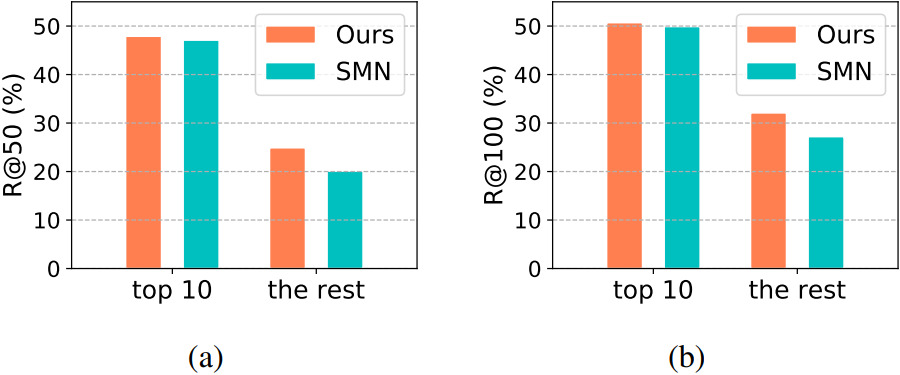
\includegraphics[width=0.6\linewidth]{fig_1.png}
  \caption{(a) Recall@50 and (b) Recall@100 of our proposed method and the SMN
    on the scene graph classification task on the Visual Genome dataset. Both
    models are trained on the whole training set and evaluated on the two
    subsets, respectively. Note that SMN is the previous best-performing
    method.}%
  \label{fig:1}
\end{figure}

As shown in \Fig{1}, current best-performing method (\textit{i.e.},
\href{https://rowanzellers.com/neuralmotifs/}{SMN}) can achieve competitive
performance if it has sufficient training samples, but its performance suffers
from a severe drop otherwise.

Objects in visual scene commonly have strongly structured regularities
(according to SMN).

A novel Knowledge-Embedded Routing Network (KERN) is introduced, which
captures the interplay of target objects and their relationships under the
explicit guidance of prior statistical knowledge and automatically mines
contextual cues to facilitate scene graph generation.

Existing works utilize the recall@$K$ (short as R@$K$, according to
\href{https://cs.stanford.edu/people/ranjaykrishna/vrd/}{VRD}) as the
evaluation metric. 

\begin{textbox}{\textit{Original Texts}}
However, this metric is easily dominated by the performance of the
relationships with a large proportion of samples. As the distribution of
different relationships is severely uneven, if one method performs well on
several most frequent relationships, it can achieve a high R@$K$ score. Thus,
it can not well measure the performance of all relationships.
\end{textbox}

A mean R@$K$ is proposed as complimentary evaluation metric:
%
\begin{enumerate}
  \item computes the R@$K$ for samples of each relationships
  \item averages over all relationships to obtain mR@$K$
\end{enumerate}

The KERN model improves the mR@50 and mR@100 from 15.4\% and 20.6\% to 19.8\%
and 26.2\% on the scene graph classification task, with relative improvements
of 28.6\% and 27.2\% respectively.

%%%%%%%%%%%%%%%%%%%%%%%%%%%%%%%%%%%%%%%%%%%%%%%%%%%%%%%%%%%%%%%%%%%%% Chapter 4
\setcounter{section}{3}
\section{Experiments}%
\label{sec:experiments}
\begin{figure}[htpb]
  \centering
  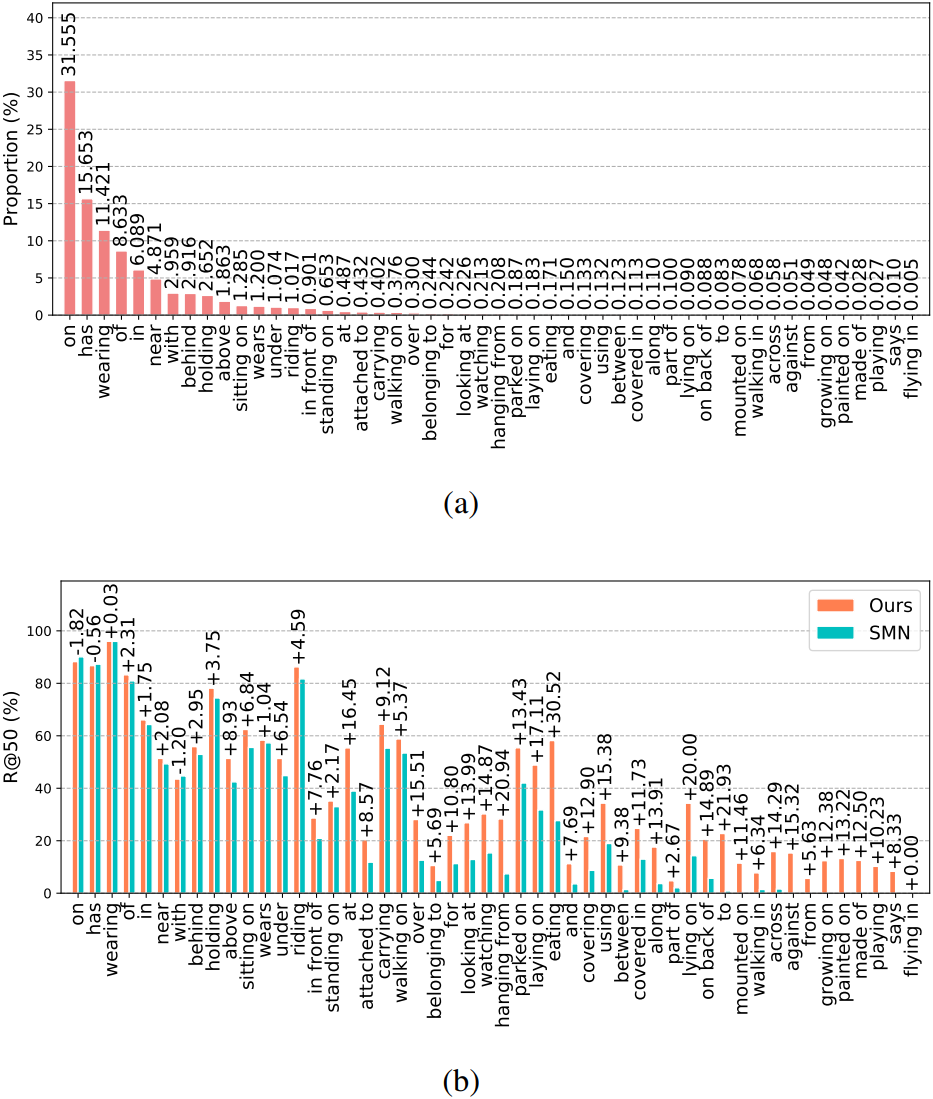
\includegraphics[width=0.8\linewidth]{fig_4.png}
  \caption{(a) The distribution of different relationships on the VG dataset.
    The training and test splits share similar distribution. (b) The R@50
    without constraint of our method and the SMN on the predicate
    classification task on the VG dataset.}%
  \label{fig:4}
\end{figure}

\end{document}
